\documentclass[border=0.2cm]{article}

\usepackage{tikz}
\usetikzlibrary{shapes.geometric}

\begin{document}
	
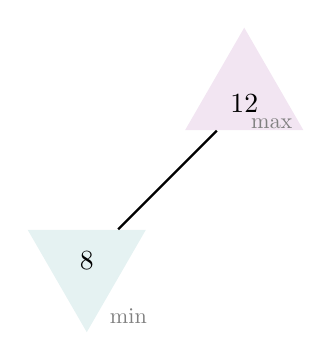
\begin{tikzpicture}
		
\tikzstyle{mytrianglemax}=[
  isosceles triangle, 
  isosceles triangle apex angle=60,
  %draw,
  shape border rotate=90,
  fill=violet!10,
  minimum size =1.3cm]	
  
\tikzstyle{mytrianglemin}=[
  isosceles triangle, 
  isosceles triangle apex angle=60,
  %draw,
  shape border rotate=-90,
  fill=teal!10,
  minimum size =1.3cm]		
	
\tikzstyle{mymax}=[above=-2pt, black!50, scale=0.8]	

\tikzstyle{mymin}=[right=2pt, black!50, scale=0.8]
	
	
% define points
\path
  (0,0) coordinate(R)
  +(-2,-2) coordinate(V1)
  ;

\node[mytrianglemax] (T) at (R) {12};
\node[mymax] at (T.315) {max};

\node[mytrianglemin] (T1) at (V1) {8};
\node[mymin] at (T1.280) {min};


% draw lines
\draw[thick]
  (T) -- (T1)
  ;

\end{tikzpicture}	
	
\end{document}